\ifx\wholebook\relax \else
% ------------------------

\documentclass[UTF8]{article}
%------------------- Other types of document example ------------------------
%
%\documentclass[twocolumn]{IEEEtran-new}
%\documentclass[12pt,twoside,draft]{IEEEtran}
%\documentstyle[9pt,twocolumn,technote,twoside]{IEEEtran}
%
%-----------------------------------------------------------------------------
\input{../../../common-en.tex}

\setcounter{page}{1}

\begin{document}

%--------------------------

% ================================================================
%                 COVER PAGE
% ================================================================

\title{The imperative red-black tree deletion algorithm}

\author{Larry~LIU~Xinyu
\thanks{{\bfseries Larry LIU} \newline
  Email: liuxinyu95@gmail.com \newline}
  }

\maketitle
\fi

\markboth{Red-black tree}{Elementary Algorithms}

\ifx\wholebook\relax
\chapter{The imperative red-black tree deletion algorithm}
\numberwithin{Exercise}{chapter}
\fi

% ================================================================
%                 Introduction
% ================================================================
\index{Red-black tree!Imperative deletion}

This appendix introduces the imperative red-black tree deletion algorithm. The idea is to perform the tree rotations and re-coloring on top of the binary search tree deletion result to adjust the balance of the tree. As mentioned in the chapter of red-black tree, the 5th red-black tree property will be violated when deleting a black node. This is because the number of black nodes in the paths through that node will reduce by one. To keep the number of black nodes unchanged, we introduce a concept of 'doubly blackness'.

\section{Doubly Black node}
\index{Reb-black tree!doubly black}

In order to realize 'doubly black' node, we need add a new color definition. As the following C++ example.

\lstset{language=C++}
\begin{lstlisting}
enum class Color { RED, BLACK, DOUBLY_BLACK };
\end{lstlisting}

When deleting a node, we re-use the binary search tree algorithm and record the parent of the deleted node. We need further processing if the deleted node is black before performing the fixing.

\begin{algorithmic}[1]
\Function{Delete}{$T, x$}
  \State $p \gets$ \Call{Parent}{$x$}
  \State $q \gets$ NIL
  \If{\Call{Left}{$x$} = NIL}
    \State $q \gets$ \Call{Right}{$x$}
    \State replace $x$ with \Call{Right}{$x$}
  \ElsIf{\Call{Right}{$x$} = NIL}
    \State $q \gets$ \Call{Left}{$x$}
    \State replace $x$ with \Call{Left}{$x$}
  \Else
    \State $y \gets$ \textproc{Min}(\Call{Right}{$x$})
    \State $p \gets$ \Call{Parent}{$y$}
    \State $q \gets$ \Call{Right}{$y$}
    \State \Call{Key}{$x$} $\gets$ \Call{Key}{$y$}
    \State copy satellite data from $y$ to $x$
    \State replace $y$ with \Call{Right}{$y$}
    \State $x \gets y$
  \EndIf
  \If{\Call{Color}{$x$} = BLACK}
    \State $T \gets$ \textproc{Delete-Fix}($T$, \Call{Make-Black}{$p$, $q$}, $q$ = NIL?)
  \EndIf
  \State release $x$
  \State \Return $T$
\EndFunction
\end{algorithmic}

The deletion algorithm takes the root $T$ and the node $x$ to be deleted. If $x$ has an empty sub-tree, we can cut off $x$, then replace it with the other sub-tree $q$. Otherwise, we locate the minimum node $y$ in the right child of $x$, then replace $x$ with $y$. We next cut off $y$ after that. If the deleted node $x$ is black, we call \textproc{Make-Black}($p$, $q$) to keep the blackness and start further processing.

\begin{algorithmic}[1]
\Function{Make-Black}{$p$, $q$}
  \If{$p$ = NIL $\land$ $q$ = NIL}
    \State \Return NIL \Comment{Returns empty if delete a singleton leaf.}
  \ElsIf{$q$ = NIL}
    \State $n \gets$ Doubly Black NIL
    \State \Call{Parent}{$n$} $\gets p$
    \State \Return $n$
  \Else
    \State \Return \Call{Blacken}{$q$}
  \EndIf
\EndFunction
\end{algorithmic}

If both $p$ and $q$ passed to \textproc{Make-Black} are empty, we are deleting the only leaf node from a singleton tree. It becames empty as the result. If the parent $p$ isn't empty, but $q$ is, it means we deleted a black leaf node, and used the NIL node to replace that black node. According to the red-black tree property 3, NIL node is black. We can change the NIL node to 'doubly black' NIL to retain the number of black nodes for all the paths through that node. Otherwise, if both $p$ and $q$ are not empty, we call \textproc{Blacken} procedure, if $q$ is red, then we color it to black; if it is already black, we color it to doubly black.

In order to resume all the red-black tree properties, we next get rid of the doubly blackness by tree rotations and re-coloring. There are three different cases (pp292 in \cite{CLRS}). The doubly black node can either be normal node or NIL node in all the cases.

\subsection{The doubly black node has a black sibling, and one of its nephew is red.}
We can rotate the tree to fix the doubly black. There are 4 sub-cases, all can be transformed to a uniformed structure as shown in figure \ref{fig:del-case}.

\begin{figure}[htbp]
   \centering
   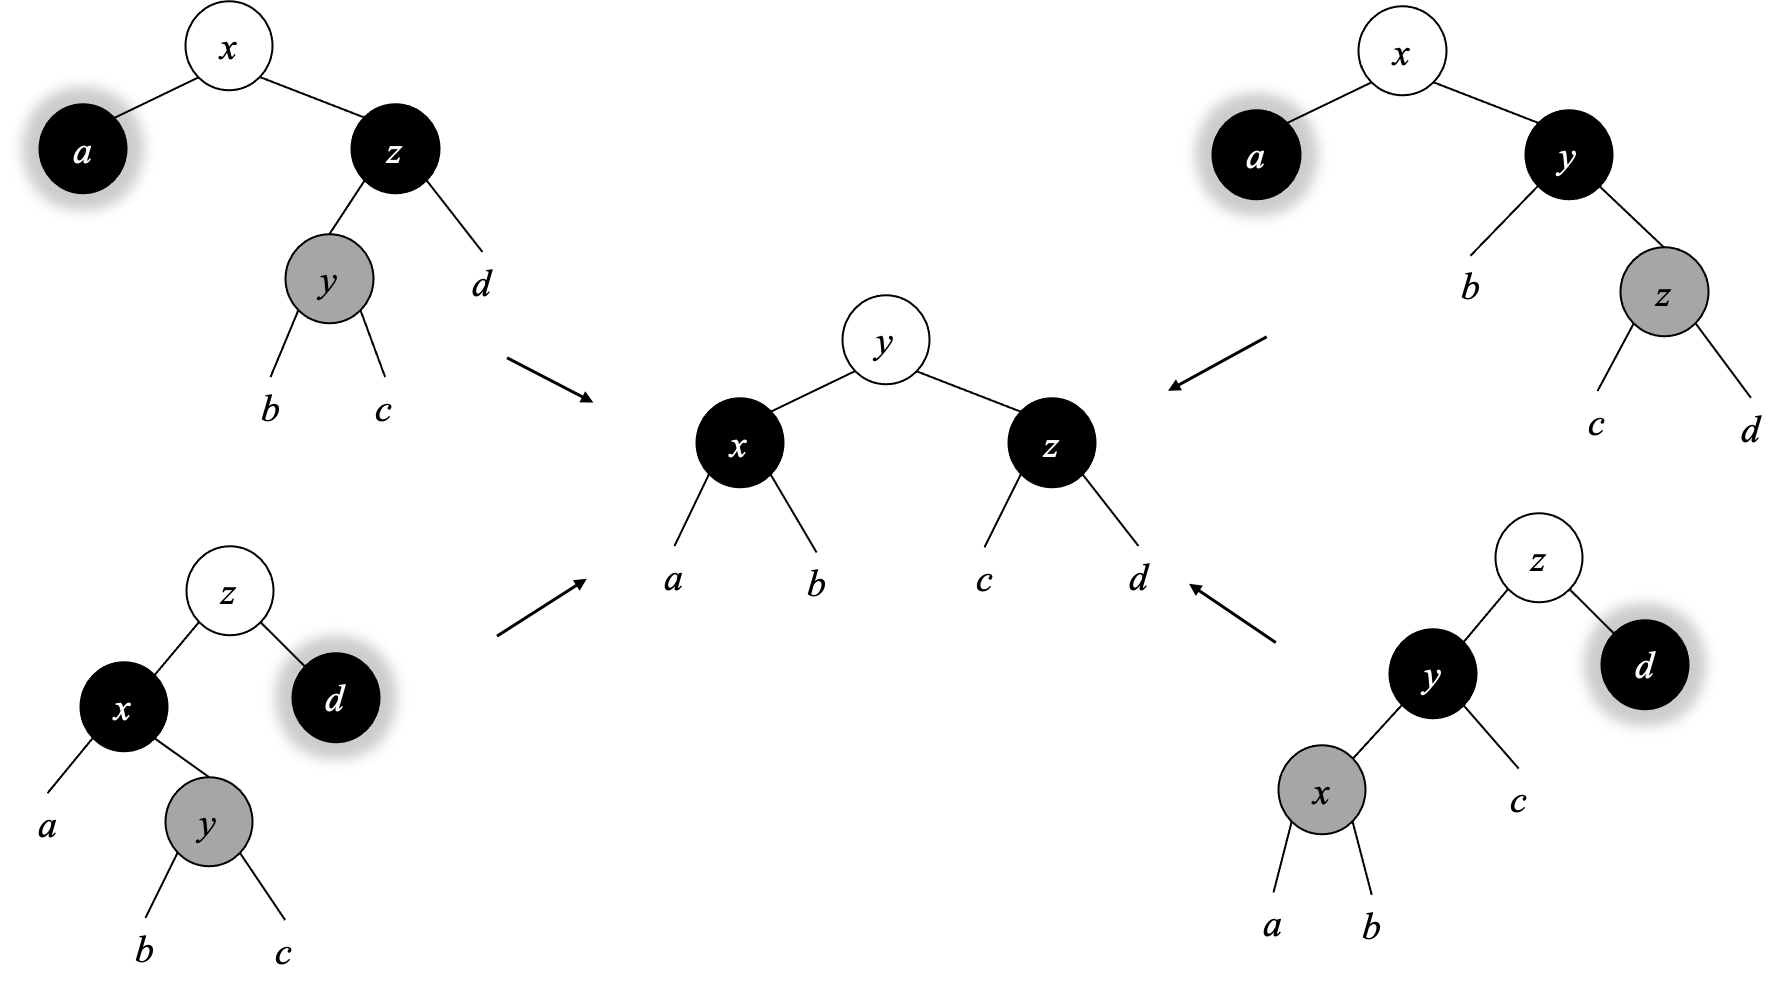
\includegraphics[scale=0.4]{../../../datastruct/tree/red-black-tree/img/del-case1.eps}
   \caption{The doubly black node has a black sibling, and one of its nephew is red. It can be fixed with a rotation.}
   \label{fig:del-case1}
\end{figure}

The following algorithm realized this fixing.

\begin{algorithmic}[1]
\Function{Delete-Fix}{$T$, $x$, $f$}
  \State $n \gets$ NIL
  \If{$f$ = True}  \Comment{$x$ is a doubly black NIL}
    \State $n \gets x$
  \EndIf
  \If{$x$ = NIL} \Comment{Delete the singleton leaf}
    \State \Return NIL
  \EndIf
  \While{$x \neq T \land$ \Call{Color}{$x$} $= \mathcal{B}^2$}
    \Comment{$x$ isn't root and is doubly black}
    \If{\Call{Sibling}{$x$} $\neq$ NIL} \Comment{The sibling isn't empty}
        \State $s \gets$ \Call{Sibling}{$x$}
        \State ...
        \If{$s$ is black $\land$ \Call{Left}{$s$} is red}
          \Comment{The sibling is black, a nephew is red}
          \If{$x = $ \textproc{Left}(\Call{Parent}{$x$})}
            \Comment{$x$ is the left}
            \State set $x$, \Call{Parent}{$x$}, and \Call{Left}{$s$} all black
            \State $T \gets$ \Call{Rotate-Right}{$T$, $s$}
            \State $T \gets$ \textproc{Rotate-Left}($T$, \Call{Parent}{$x$})
          \Else \Comment{$x$ is the right}
            \State set $x$, \Call{Parent}{$x$}, $s$, and \Call{Left}{$s$} all black
            \State $T \gets$ \textproc{Rotate-Right}($T$, \Call{Parent}{$x$})
          \EndIf
        \ElsIf{$s$ is black $\land$ \Call{Right}{$s$} is red}
          \Comment{The sibling is black, a nephew is red}
          \If{$x = $ \textproc{Left}(\Call{Parent}{$x$})} \Comment{$x$ is the left}
            \State set $x$, \Call{Parent}{$x$}, $s$, and \Call{Right}{$s$} all black
            \State $T \gets$ \textproc{Rotate-Left}($T$, \Call{Parent}{$x$})
          \Else \Comment{$x$ is the right}
            \State set $x$, \Call{Parent}{$x$}, and \Call{Right}{$s$} all black
            \State $T \gets$ \Call{Rotate-Left}{$T$, $s$}
            \State $T \gets$ \textproc{Rotate-Right}($T$, \Call{Parent}{$x$})
          \EndIf
        \State ...
        \EndIf
    \EndIf
  \EndWhile
\EndFunction
\end{algorithmic}

\subsection{The sibling of the doubly black node is red.}

We can rotate the tree to change the doubly black node to normal black node. As shown in figure \ref{fig:del-case2}, after transform from the left to the right structure, we can re-color node $a$ or $c$ to black.

\begin{figure}[htbp]
  \centering
  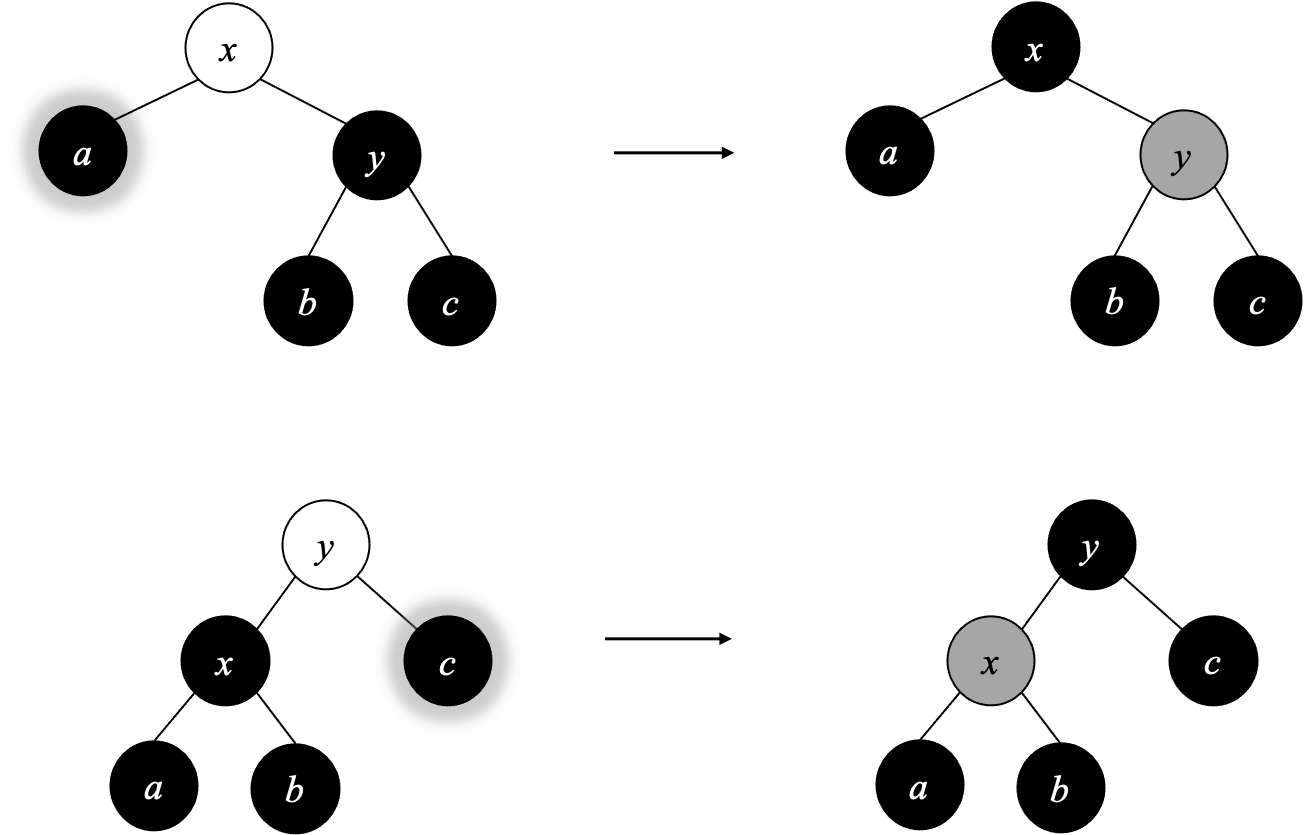
\includegraphics[scale=0.4]{../../../datastruct/tree/red-black-tree/img/del-case3.eps}
  \caption{The sibling of the doubly black node is red} \label{fig:del-case2}
\end{figure}

We can add this fixing on top of the previous algorithm.

\begin{algorithmic}[1]
\Function{Delete-Fix}{$T$, $x$, $f$}
  \State $n \gets$ NIL
  \If{$f$ = True}  \Comment{$x$ is a doubly black NIL}
    \State $n \gets x$
  \EndIf
  \If{$x$ = NIL} \Comment{Delete the singleton leaf}
    \State \Return NIL
  \EndIf
  \While{$x \neq T \land$ \Call{Color}{$x$} $= \mathcal{B}^2$}
    \Comment{$x$ isn't root and is doubly black}
    \If{\Call{Sibling}{$x$} $\neq$ NIL} \Comment{The sibling isn't empty}
        \State $s \gets$ \Call{Sibling}{$x$}
        \If{$s$ is red} \Comment{The sibling is red}
          \State set \Call{Parent}{$x$} red
          \State set $s$ black
          \If{$x = $ \textproc{Left}(\Call{Parent}{$x$})} \Comment{$x$ is the left}
            \State $T \gets$ \textproc{Rotate-Left}{$T$, \Call{Parent}{$x$}}
          \Else \Comment{$x$ is the right}
            \State $T \gets$ \textproc{Rotate-Right}{$T$, \Call{Parent}{$x$}}
          \EndIf
        \ElsIf{$s$ is black $\land$ \Call{Left}{$s$} is red}
          \Comment{THe sibling is black, a nephew is red}
          \State ...
        \EndIf
    \EndIf
  \EndWhile
\EndFunction
\end{algorithmic}

\subsection{The sibling of the doubly black node, and both nephews are black.}
In this case, we can re-color the sibing to red, change the doubly black node back to black, then propagate the doubly blackness to the parent in upper level. As shown in figure \ref{fig:del-case3}, there are two symetric sub-cases.

\begin{figure}[htbp]
  \centering
  \setlength{\unitlength}{1cm}
  \begin{picture}(10, 4)
  \put(5, 2){$\Rightarrow$}
  \subfloat[$x$ is red or black.]{\includegraphics[scale=0.4]{../../../datastruct/tree/red-black-tree/img/case2-a.ps}}
  \subfloat[Change $x$ to black if it's red, otherwise change it to doubly black.]{\includegraphics[scale=0.4]{../../../datastruct/tree/red-black-tree/img/case2-a1.ps}}
  \end{picture}
  \\
  \begin{picture}(10, 5)
  \put(5, 2){$\Rightarrow$}
  \subfloat[$y$ is red or black.]{\includegraphics[scale=0.4]{../../../datastruct/tree/red-black-tree/img/case2-b.ps}}
  \subfloat[Change $y$ to black if it's red, otherwsie change it to doubly black.]{\includegraphics[scale=0.4]{../../../datastruct/tree/red-black-tree/img/case2-b1.ps}}
  \end{picture}
  \\
  \begin{picture}(1, 0.5)\end{picture} %pad
  \caption{Propagate the doubly blackness upward} \label{fig:del-case3}
\end{figure}

The sibling of the doubly black node isn't empty in all the 3 cases. If the sibling is empty, we can change the doubly black node back to back, and propagate the blackness upward. If the doubly blackness reach the root, we can change the root to black to terminate the fixing process. It can also terminate if the doubly black node is re-colored in the midway. At last of the algorithm, if the doubly black node passed in is a doubly black empty node, we turn it back to normal NIL node. The complete altorithm is given as below.

\begin{algorithmic}[1]
\Function{Delete-Fix}{$T$, $x$, $f$}
  \State $n \gets$ NIL
  \If{$f$ = True}  \Comment{$x$ is a doubly black NIL}
    \State $n \gets x$
  \EndIf
  \If{$x$ = NIL} \Comment{Delete the singleton leaf}
    \State \Return NIL
  \EndIf
  \While{$x \neq T \land$ \Call{Color}{$x$} $= \mathcal{B}^2$}
    \Comment{$x$ isn't root and is doubly black}
    \If{\Call{Sibling}{$x$} $\neq$ NIL} \Comment{The sibling isn't empty}
        \State $s \gets$ \Call{Sibling}{$x$}
        \If{$s$ is red} \Comment{The sibling is red}
          \State set \Call{Parent}{$x$} red
          \State set $s$ black
          \If{$x = $ \textproc{Left}(\Call{Parent}{$x$})} \Comment{$x$ is the left}
            \State $T \gets$ \textproc{Rotate-Left}{$T$, \Call{Parent}{$x$}}
          \Else \Comment{$x$ is the right}
            \State $T \gets$ \textproc{Rotate-Right}{$T$, \Call{Parent}{$x$}}
          \EndIf
        \ElsIf{$s$ is black $\land$ \Call{Left}{$s$} is red}
          \Comment{The sibling is black, a nephew is red}
          \If{$x = $ \textproc{Left}(\Call{Parent}{$x$})}
            \Comment{$x$ is the left}
            \State set $x$, \Call{Parent}{$x$}, and \Call{Left}{$s$} all black
            \State $T \gets$ \Call{Rotate-Right}{$T$, $s$}
            \State $T \gets$ \textproc{Rotate-Left}($T$, \Call{Parent}{$x$})
          \Else \Comment{$x$ is the right}
            \State set $x$, \Call{Parent}{$x$}, $s$, and \Call{Left}{$s$} all black
            \State $T \gets$ \textproc{Rotate-Right}($T$, \Call{Parent}{$x$})
          \EndIf
        \ElsIf{$s$ is black $\land$ \Call{Right}{$s$} is red}
          \Comment{The sibling is black, a nephew is red}
          \If{$x = $ \textproc{Left}(\Call{Parent}{$x$})}
            \Comment{$x$ is the left}
            \State set $x$, \Call{Parent}{$x$}, $s$, and \Call{Right}{$s$} all black
            \State $T \gets$ \textproc{Rotate-Left}($T$, \Call{Parent}{$x$})
          \Else \Comment{$x$ is the right}
            \State set $x$, \Call{Parent}{$x$}, and \Call{Right}{$s$} all black
            \State $T \gets$ \Call{Rotate-Left}{$T$, $s$}
            \State $T \gets$ \textproc{Rotate-Right}($T$, \Call{Parent}{$x$})
          \EndIf
        \ElsIf{$s$, \Call{Left}{$s$}, and \Call{Right}{$s$} are all black}
          \Comment{The sibling and nephews are all black}
          \State set $x$ black
          \State set $s$ red
          \State \textproc{Blacken}(\Call{Parent}{$x$})
          \State $x \gets$ \Call{Parent}{$x$}
        \EndIf
    \Else \Comment{No sibling, propagate the blackness upward}
      \State set $x$ black
      \State \textproc{Blacken}(\Call{Parent}{$x$})
      \State $x \gets$ \Call{Parent}{$x$}
    \EndIf
  \EndWhile
  \State set $T$ black
  \If{$n \neq$ NIL} \Comment{Replace the doubly black NIL with normal NIL}
    \State replace $n$ with NIL
  \EndIf
  \State \Return $T$
\EndFunction
\end{algorithmic}

When fixing the deltion result, we passed in the root $T$; the node (can be doubly black) to be fixed as $x$; and a flag $f$. The flag is true if the node to be fixed $x$ is doubly black NIL. We record the doubly black NIL with $n$, and replace $n$ with the normal NIL after fixing.

The following is the example deletion program in C++.

\lstset{language=C++}
\begin{lstlisting}
Node* del(Node* t, Node* x) {
    if (!x) return t;
    Node* parent = x->parent;
    Node* db = nullptr;        //doubly black
    Node* y;

    if (x->left == nullptr) {
        db = x->right;
        x->replaceWith(db);
    } else if (x->right == nullptr) {
        db = x->left;
        x->replaceWith(db);
    } else {
        y = min(x->right);
        parent = y->parent;
        db = y->right;
        x->key = y->key;
        y->replaceWith(db);
        x = y;
    }
    if (x->color == Color::BLACK)
        t = deleteFix(t, makeBlack(parent, db), db == nullptr);
    remove(x);
    return t;
}
\end{lstlisting}

Where \texttt{makeBlack} check if the node change to doubly black after deletion, and handle the special case of doubly black NIL.

\begin{lstlisting}
Node* makeBlack(Node* parent, Node* x) {
    if (!parent && ! x)
        return nullptr;
    if (!x)
        return Node::replace(parent, x, new Node(0, Color::DOUBLY_BLACK));
    return blacken(x);
}
\end{lstlisting}

The function \texttt{replace(parent, x, y)} replaces the child of the \texttt{parent}, which is \texttt{x}, with the node \texttt{y}.

\begin{lstlisting}
static Node* replace(Node* parent, Node* x, Node* y) {
    if (parent == nullptr) {
        if (y) y->parent = nullptr;
    } else if (parent->left == x) {
        parent->setLeft(y);
    } else {
        parent->setRight(y);
    }
    if (x) x->parent = nullptr;
    return y;
}
\end{lstlisting}

The function \texttt{blacken(node)} re-colors the red node to black, and re-colors the black node to doubly black.

\begin{lstlisting}
Node* blacken(Node* x) {
    x->color = isRed(x) ? Color::BLACK : Color::DOUBLY_BLACK;
    return x;
}
\end{lstlisting}

Below is the final fixing process.

\begin{lstlisting}
Node* deleteFix(Node* t, Node* db, bool isDBEmpty) {
    Node* dbEmpty = isDBEmpty ? db : nullptr;
    if (!db) return nullptr;    // remove the root from a leaf tree;
    while (db != t && db->color == Color::DOUBLY_BLACK) {
        if (db->sibling() != nullptr) {
            if (isRed(db->sibling())) {
                // the sibling is red, (transform to make the sibling black)
                setColors(db->parent, Color::RED,
                          db->sibling(), Color::BLACK);
                if (db == db->parent->left)
                    t = leftRotate(t, db->parent);
                else
                    t = rightRotate(t, db->parent);
            } else if (isBlack(db->sibling()) && isRed(db->sibling()->left)) {
                // the sibling is black, and one nephew is red
                if (db == db->parent->left) {
                    setColors(db, Color::BLACK,
                              db->parent, Color::BLACK,
                              db->sibling()->left, db->parent->color);
                    t = rightRotate(t, db->sibling());
                    t = leftRotate(t, db->parent);
                } else {
                    setColors(db, Color::BLACK,
                              db->parent, Color::BLACK,
                              db->sibling(), db->parent->color,
                              db->sibling()->left, Color::BLACK);
                    t = rightRotate(t, db->parent);
                }
            } else if (isBlack(db->sibling()) && isRed(db->sibling()->right)) {
                if (db == db->parent->left) {
                    setColors(db, Color::BLACK,
                              db->parent, Color::BLACK,
                              db->sibling(), db->parent->color,
                              db->sibling()->right, Color::BLACK);
                    t = leftRotate(t, db->parent);
                } else {
                    setColors(db, Color::BLACK,
                              db->parent, Color::BLACK,
                              db->sibling()->right, db->parent->color);
                    t = leftRotate(t, db->sibling());
                    t = rightRotate(t, db->parent);
                }
            } else if (isBlack(db->sibling()) &&
                       isBlack(db->sibling()->left) &&
                       isBlack(db->sibling()->right)) {
                // the sibling and both nephews are black.
                // move the blackness up
                setColors(db, Color::BLACK,
                          db->sibling(), Color::RED);
                blacken(db->parent);
                db = db->parent;
            }
        } else { // no sibling, move the blackness up
            db->color = Color::BLACK;
            blacken(db->parent);
            db = db->parent;
        }
    }
    t->color = Color::BLACK;
    if (dbEmpty) { // change the doubly black nil to nil
        dbEmpty->replaceWith(nullptr);
        delete dbEmpty;
    }
    return t;
}
\end{lstlisting}

Where \texttt{isBlack(node)} tests if a node is black, the NIL node is also black according to the red-black tree property.

\begin{lstlisting}
bool isBlack(Node* x) {
    return x == nullptr || x->color == Color::BLACK;
}

bool isRed(Node* x) {
    return x != nullptr && x->color == Color::RED;
}
\end{lstlisting}

The \texttt{setColors} is a set of auxiliary functions to re-color nodes.

\begin{lstlisting}
void setColors(Node* x, Color a, Node* y, Color b) { x->color = a; y->color = b; }

void setColors(Node* x, Color a, Node* y, Color b, Node* z, Color c) {
    setColors(x, a, y, b);
    z->color = c;
}

void setColors(Node* x, Color a, Node* y, Color b,
               Node* z, Color c, Node* q, Color d) {
    setColors(x, a, y, b);
    setColors(z, c, q, d);
}
\end{lstlisting}

Before returning the final result, the algorithm check the doubly black NIL, it calls the \texttt{replaceWith} method of the node, which is implemented with the \texttt{replace} function defined previously.

\begin{lstlisting}
void replaceWith(Node* y) {
    replace(parent, this, y);
}
\end{lstlisting}

The algorithm terminates when reach the root or the doubly blackness is eliminated. Consider the red-black tree is balanced, the deletion algorithm is bound to $O(\lg n)$ time for the tree contains $n$ nodes.

\begin{Exercise}

\begin{itemize}
\item Implement the red-black tree deletion algorithm in an imperative programming langauge.
\item Write a program in an imperative programming language to test if a given tree satisfies the 5 red-black tree properties. Use this program to verify the red-black tree deletion algorithm.
\end{itemize}

\end{Exercise}

\ifx\wholebook\relax \else
\begin{thebibliography}{99}

\bibitem{CLRS}
Thomas H. Cormen, Charles E. Leiserson, Ronald L. Rivest and Clifford Stein.
``Introduction to Algorithms, Second Edition''. ISBN:0262032937. The MIT Press. 2001

\end{thebibliography}

\end{document}
\fi
